%% *************************************************************************
%%
%% This is an RIT Space Exploration Standard defining guidelines for content
%% and formatting of project design documents.
%%
%% This document uses IEEEtran.cls, the official IEEE LaTeX class
%% for authors of the Institute of Electrical and Electronics Engineers
%% (IEEE) Transactions journals and conferences.
%%
%% *************************************************************************

%% *************************************************************************
% LaTeX REFERENCES
% ----------------
%   Intro to LaTeX: http://www.rpi.edu/dept/arc/docs/latex/latex-intro.pdf
%   Comprehensive LaTeX symbol list: http://tug.ctan.org/info/symbols/comprehensive/symbols-a4.pdf
%% *************************************************************************

\documentclass[conference]{IEEEtran} % http://www.ctan.org/pkg/ieeetran
\usepackage{blindtext}
\usepackage{graphicx}
\usepackage{nomencl}
\usepackage{siunitx}
\usepackage{hyperref}
\usepackage[T1]{fontenc}
\usepackage{etoolbox}

\makenomenclature{}

\title{RIT Space Exploration Project Design Document Standard Format and Sample Content}


\author {
  \IEEEauthorblockN{% This block is for author Names.
    Austin~Bodzas\IEEEauthorrefmark{1}
  }
  \IEEEauthorblockA{% This block is for the author Affiliations, aka department and university
    RIT Space Exploration, Rochester Institute of Technology \\ %\\ starts a new line
    Rochester, N.Y. \\
    Email:
    \IEEEauthorrefmark{1}abb6499@rit.edu
  }
}
% page header for pages other than cover page
\markboth{Microhab}%
{Bodzas \MakeLowercase{\textit{et al.}}: RIT Space Exploration}

% Initial setup is over, start building the document itself
\begin{document}
\maketitle%
% correct bad hyphenation here, separated by spaces
\hyphenation{explor-ation}

\begin{abstract}

      % The abstract is a brief summary of the design document. Typically it includes the purpose of the design document, key goals or objectives, and justifications.
      % Be sure not to confuse the abstract with the introduction.
      % It is easiest to write the abstract after the rest of the paper has been written.
      % That way you can choose key information from the sections that you've already completed and string them together in the abstract.
      % Consider the abstract to be your elevator pitch to anyone reading this design document.
      % What are they reading?
      % What is the goal?
      % Why is it worth my time?
      % The abstract is what will show up in Google results and other search engines, and what people will read when they are deciding what is worth their time and brain power.
    A project definition for the Microhab project.  Microhab is the term the
    HAB team has been using to describe a smaller balloon and payload than is
    typically used by the group (1200 grams). However, this project expands upon
    the term with the main goal of minimizing costs that go into building and
    launching a HAB.\@
\end{abstract}

\label{sec:nomenclature}
\newcommand{\nomunit}[1]{%
\renewcommand{\nomentryend}{\hspace*{\fill}#1}}
\renewcommand{\nompreamble}{
    % If you include mathematical expressions or express variables in the design document, list them with their corresponding definitions here as a list.
    % The two lines below make it look nice when defining units/values to constants.

    % Note that math terms and non-math terms are separated and alphabetized, regardless of the order in which they are defined. (Recall terms \$like this\$ are in the math environment)
    % Read more about advanced nomenclature formatting here:\\
    % \url{https://www.sharelatex.com/learn/Nomenclatures}
  }
\nomenclature{RIT}{Rochester Institute of Technology}
\nomenclature{SPEX}{RIT Space Exploration}
\nomenclature{PDD}{Project Design Document}
% Below are examples of using nomenclature for math symbols and constants or units
% \nomenclature{$\dot{m}$}{Mass flow rate
%   \nomunit{\,\si{\kilo\gram\per\second}}}
% \nomenclature{$c$}{Speed of light
%  \nomunit{\,\SI{2.9979e8}{\meter\per\second}}}
\printnomenclature{}


% HELPFUL HINT: If you get the warning ``Command terminated with space.'' when using a \command try placing ``%'' or ``{}'' immediately following the command.

% The sections included here are required. Additional sections and subsections may be added as necessary.
\section{Introduction}
\label{sec:introduction}
  % The introduction is a place to give background and context before diving into the subject matter.
  % Establish context for the work you are about to propose and the main ideas of the proposition itself.

\IEEEPARstart{T}{raditional} HAB launches are very expensive for the SPEX team.
A large 1200g balloon can cost, at a minimum, over 125USD.  Helium tank fills,
which these launches require a full fill, can cost over 200USD. These two costs
are a definite non-reusable resource. An avionics package consisting of COTS
Arduino, breakout sensors, and a large battery pack can easily add up to over
90USD. The avionics hardware can be reused but every launch should be assumed a
one time only use of hardware due to high risks of losing the payload.

Microhab will reduce the costs of these three large costs that make frequent HAB
launches unaffordable for undergraduate research. A smaller, simpler, more
focused payload will result in cheaper avionics hardware costs. A lighter
payload also doesn't require such a large balloon, enabling a cheaper, smaller
balloon and orders of magnitude less helium use per launch.

\section{Primary Objective}
\label{sec:primary-obj}
  % At the end of the day, whether the project ``succeeds'' or ``fails'' is judged against the objectives it sought to meet.
  % Note that results that contradict expectations/hypotheses are not failures if the scientific \& engineering methods are followed along the way.
  % Sometimes our expectations are wrong and that can be just as successful as getting data we thought we'd see.
  % What matters are what questions you intend to answer.
  % This is the main purpose or main goal the project hopes to achieve.

The SPEX Standard defines format and style guidelines for project documentation. The Project Design Document Standard controls these guidelines as applicable to young, exploratory ideas.

The ultimate goal of a PDD is to capture all ideas (including ones that are beyond our capability, interesting ideas, or things we just dont have time for, in addition to the ones that we actually work on and develop) and archive them such that if a student goes on coop or graduates, these ideas would not leave with them.

\begin{figure}
  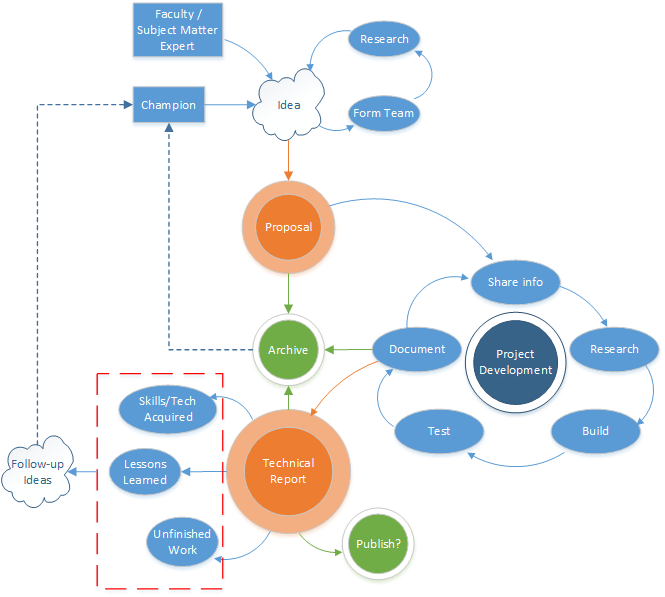
\includegraphics[width=\linewidth]{figs/project-life-cycle.png}
  \caption{A PDD is the first piece of documentation to be archived in the project life cycle. Since the life cycle can be iterative, a new design document may also refer to one or more previous SPPs.}
\label{fig:lifecycle}
\end{figure}

% \section{Secondary Objectives}
% \label{sec:secondary-obj}
% Secondary Objectives are lower priority or bonus objectives that are significant but not the main focus of the project. This template does not have secondary objectives.

\section{Benefit to SPEX}
\label{sec:benefit}
% One of the core values of SPEX is to provide opportunities for academic and professional growth for its members,
% and to challenge them with interesting projects.
% In this section, explain how the project would benefit SPEX members as students,
% space enthusiasts, and young professionals.

By writing design documents and familiarizing undergraduate and graduate students from any discipline with this type of approach and execution, SPEX members will be better equipped convey their ideas to others in a methodical and organized manner.
Ideally, an abundance of ideas and projects encapsulated in PDDs would outlive their respective authors and continue to sustain SPEX with valuable research opportunities invariant of individual members' absences due to co-ops or graduations.
Perhaps in the future, SPEX design documents may be used as baselines for grant applications and other funded research efforts.


% Below I have used subsections to identify key ideas in this section. These particular subsections are not required as part of the SPEX Standard, but serve as an example of using subsections in a text.

\subsection{Mindset}
\label{subsec:mindset}
Firstly, it gets people in the right mindset for thinking about what is important and what needs to be considered before taking off on a project.
Publishing a PDD imbues a sense of formality that hopefully makes its way into the level of seriousness and merit that is desirable for SPEX to pursue.

\subsection{Traceability}
\label{subsec:traceability}
Similarly, a PDD serves to provide the foundation for traceability in requirements and objectives to projects as they grow and change.
This prevents blockers such as feature creep, rabbit holes, and spun tires, and hopefully prevents good projects from dying by getting too off track.

\subsection{Accessibility}
\label{subsec:plug-n-play}
  % Note below that LaTeX uses weird formatting when it comes to quotation marks.
  % The style below is correct to display forward quotes `` at the start of the phrase and backquotes '' at the end.

Having a ``plug-and-play'' template is the first step to learning how to one's own SPP\@.
It removes a major barrier of starting from scratch, providing example content to which one could refer when creating their own.
\LaTeX{} may prove to be daunting for some people, but it is arguably better to encourage people to learn LaTeX than to rely on something like Microsoft Word.

\section{Implementation}
\label{sec:implementation}
  % What path do you anticipate the project to take?

In the ideal case, every project begins with a design document.
That design document gets sent around to SPEX members (and non-members) to draw support and build a team.
Research and work takes place, documented along the way until  an ending point is reached (e.g.\ project completion, end of the semester, team attrition, etc.).

At the end of the project (or end of semester, whichever comes first), the team writes a report of the project with what they did, if it was successful, and recommendations for future projects.
A future SPEX member might pick up where the last paper left off, and the cycle repeats.

\subsection{Deliverables}
\label{subsec:deliverables}
  % When all is said and done, what will you have to show for it?
  % Examples: Hardware, software, poster, ImagineRIT demo, presentations, technical papers...
Physical or intellectual property may constitute a project's deliverables.
Test articles, test stands, and other hardware, software, as well as posters, presentations or other reports are all valid deliverables.
Not all deliverables may be known at the time of writing a PDD, but at least several key deliverables should be identified at the start of a project.
This helps guide the final outcome and is a fundamental part of a project's life cycle.

\subsection{Milestones}
\label{subsec:milestones}
  % Be as detailed as you can, but it's okay if there are unknowns.
  % At the very least, specify how many semester you expect the project to take until it reaches completion.
Deadlines and milestones provide clear goals from which timelines and schedules may be developed, and also set up a project for a series of ``sanity checks'' along the project's development cycle.
Early on, these milestones include design reviews on system and subsystem levels.
Later, milestones are usually important tests or experiments.
Events such as ImagineRIT may also serve as milestones to mark a project's development progress or completion.

\section{Externalities}
  % Things not directly related to the work or outcomes, but related to the project as a whole.
\subsection{Prerequisite Skills}
  % Which skills do team members need to have before work can start (not including skills that will be learned ``on the job'')?
It is obvious that team members will learn certain skills as a project progresses, but there are always some tasks that require a minimum skill level to provide meaningful contributions to a project's development.
These prerequisite skills are best identified by examining past projects and discussing the project with faculty or subject matter experts.
It is strongly recommended to be conservative in skill estimation.
Underestimate team member skill levels and overestimate the challenge.
Many projects have failed because the team overestimated their own abilities or underestimated the difficulty of their project.

\subsection{Funding Requirements}
  % Estimate costs that would be needed to meet objectives.
Like prerequisite skills, it is wise to overestimate the cost of components, materials and other resources that a project requires.
For physical projects, costs may be estimated by benchmarking the costs of similar systems or determining a representative bill of materials and using the aggregate cost of its items.

\subsection{Faculty Support}
  % Identify faculty that will be involved (or would need to be involved) to meet objectives.
  % Note that if a professor is the Principal Investigator (P.I.) for a project, there still needs to be a student as the SPEX Project Champion.
Support from university faculty is almost always essential to a project's success.
Faculty provide not only guidance and subject matter expertise, but may also connect a team with resources and networking opportunities.
SPEX projects do not require faculty support, but it is highly recommended to identify professors with an interest or expertise in a project as early as possible.

\subsection{Long-Term Vision}
\label{sec:vision}
As SPEX student members get more experience writing these papers, the group will build a library of meaningful work and be able to save it in an organized manner.
Knowledge will be preserved and easily shared.
Perhaps Project Design Document could eventually get published, in a journal or otherwise\ldots

\section*{Acknowledgements}
The author would like to thank Dr.~Bill Destler and Rebecca Johnson for being exemplary humans, Anthony Hennig for founding RIT Space Exploration, and all the SPEX members that continue to invest their time and energy into the pursuit of space exploration.

\onecolumn
\appendices{}
\section{Project Life Cycle}
\begin{figure}[h]
  \centering
  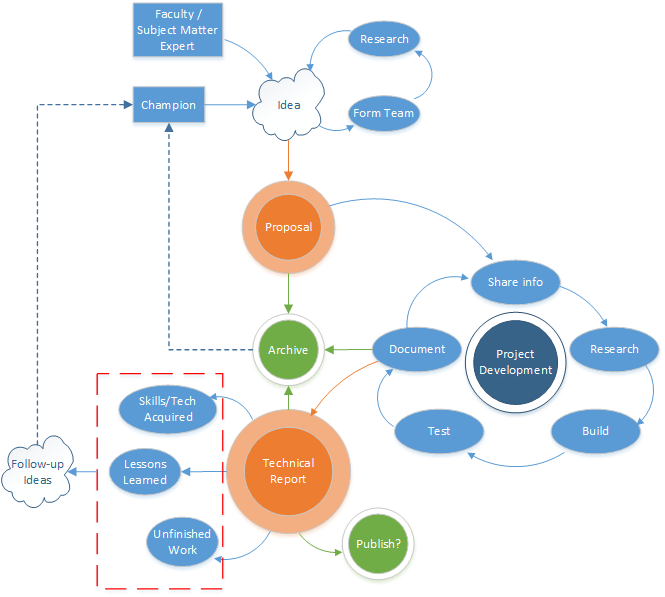
\includegraphics[]{figs/project-life-cycle.png}
  \caption{Enlarged version of the diagram in \autoref{fig:lifecycle}.}
\end{figure}

\end{document}
